\subsection{Redes Neurais Artificiais}

Em experimentos iniciais, os resultados indicaram uma classificação ruim e inconsistente, e uma análise mais profunda indicou que a otmização da função custo apresentava uma considerável demora para convergir. Um modo de corrigir esse problema é a normalização do conjunto de dados \cite{backprop}. Testes com a aplicação dessa técnica apontaram resultados melhores e mais consistentes, portanto decidiu-se pela aplicação de normalização.

Foram realizados testes com redução de dimensionalidade, porém a diferença no tempo dos experimentos não foi grande o suficiente pra justificar a piora nos resultados devido à perda de variância dos dados.

Um dos parâmetros do algoritmo é a quantidade de iterações para otimização da função custo. A Figura \ref{fig:grafico_nn} corresponde a uma curva que apresenta a relação entre valor da função custo e número de iterações:

\begin{figure}[ht]
  \centering
    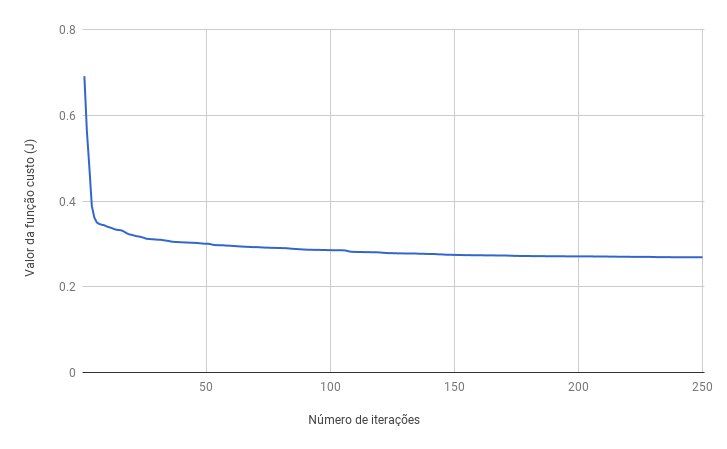
\includegraphics[width=0.5\textwidth]{chart.png}
    \caption{Curva de relação entre número de iterações e valor da função custo}
    \label{fig:grafico_nn}
\end{figure}


De acordo com a curva, foi escolhido o valor de 75 iterações, por se tratar de um ponto onde a execução não é excessiva, porém com um nível satisfatório de otimização para a função custo.

Por fim, dois parâmetros inteferem diretamente no desempenho: o número de nós na camada intermediária, e o $\lambda$ utilizado na regularização dos pesos. Para otimizá-los, foi realizada uma busca em \emph{grid}, onde os seguintes valores foram testados, utilizando o MCC como referência para comparação:

\begin{itemize}
\item Número de nós: De $3$ a $25$.
\item $\lambda$: $0, 0.01, 0,05, 0.10, 0.25, 0.5, 0.75, 1$.
\end{itemize}

Após a busca, foram os selecionados 6 nós na camada intermediária e $\lambda = 0.05$. 